\documentclass[15pt,margin=1in,innermargin=-4.5in,blockverticalspace=-0.25in]{tikzposter}
\geometry{paperwidth=42in,paperheight=30in}
\usepackage[utf8]{inputenc}
\usepackage{amsmath}
\usepackage{amsfonts}
\usepackage{amsthm}
\usepackage{amssymb}
\usepackage{mathrsfs}
\usepackage{graphicx}
\usepackage{adjustbox}
\usepackage{enumitem}
\usepackage[backend=biber,style=numeric]{biblatex}
\usepackage{emory-theme}
\renewcommand{\familydefault}{\sfdefault}

\usepackage{mwe} % for placeholder images

\addbibresource{refs.bib}

% set theme parameters
\tikzposterlatexaffectionproofoff
\usetheme{EmoryTheme}
\usecolorstyle{EmoryStyle}

\title{\textbf{Reproduction of `Multi-Task Learning using Uncertainty to Weigh Losses'}}
\author{D. Baerg, O. Key, J. Materzynska, M. Tong}
\institute{Department of Computer Science, University of Oxford}
\titlegraphic{\qquad \qquad \qquad \qquad \qquad  
\includegraphics[width=0.06\textwidth]{oxford.jpg}}

% begin document
\begin{document}
\maketitle


\centering
\begin{columns}
    \column{0.32}

    \block{A new approach to multi-task learning}{
             
        Paper on `Multi-Task Learning using Uncertainty to Weigh Losses' -- Kendall, Gal \& Cipolla, 2017.
        \begin{itemize}
        \item Principled approach to multi-task learning, demonstrated on the multi-task problem of semantic segmentation, instance segmentation and depth regression for the Cityscapes dataset
        
        \begin{tikzfigure}[Model architecture (Kendall et al., 2017)]
            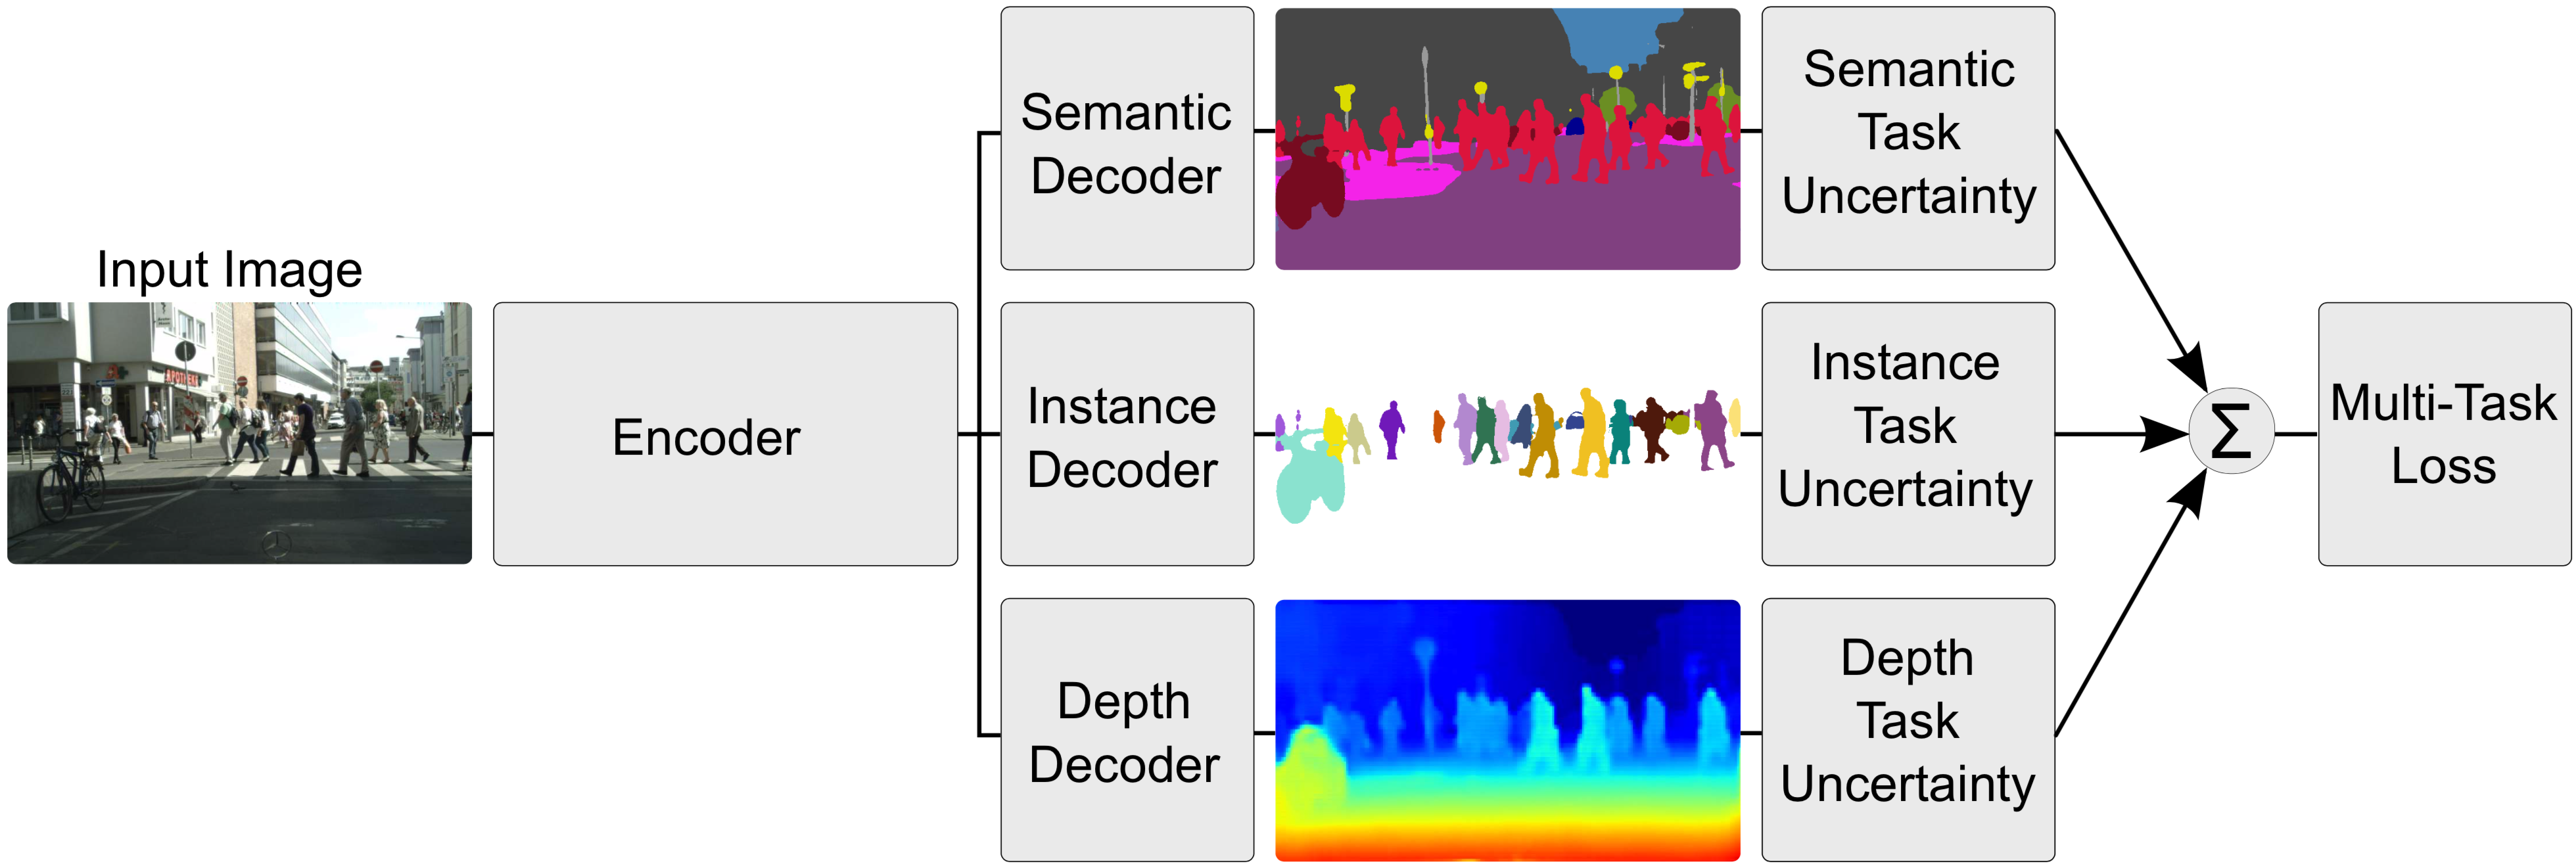
\includegraphics[width=1\linewidth]{overall}
        \end{tikzfigure}
        
        \item 3 key contributions:
        \begin{enumerate}
       \item  Aleatoric homoscedastic uncertainty to weigh losses in different tasks
       \item  Unified architecture for all three tasks with the same encoder for different tasks, with a separate decoder for each task
       \item Demonstrating that loss weighting is important for performance, and showing how superior performance can be achieved on multi-task models compared to individually trained single-task models
       \end{enumerate}
      
       \item Overall joint loss function: 
       \[ \mathcal{L} \approx 
       \frac{1}{\sigma^2_\text{sem}} \mathcal{L}_\text{sem}  + \log \sigma_\text{sem}
       + \frac{1}{2\sigma^2_\text{ins}} \mathcal{L}_\text{ins}+ \log \sigma_\text{ins}
       + \frac{1}{2\sigma^2_\text{dep}} \mathcal{L}_\text{dep}
        + \log \sigma_\text{dep} 
  \]
     
  \item Model consisted of DeepLabv3 encoder architecture, including ResNet-101 layers with dilated convolutions and Atrous Spatial Pooling Pyramid module to increase contextual awareness with a simple decoder architecture with two convolutional layers for each task
\end{itemize}
       
                    }
       
      
    
    \block{Selected reproduction objective}{
    
       \begin{itemize}
       
       \item Comparison of multi-task learning with single-task learning and learned loss weights with fixed loss weights
       \item Subsampled dataset, Tiny Cityscapes, requires less computation time
       
       \end{itemize}
    
       %\begin{tikzfigure}[Results that we aimed to reproduce (Kendall et al., 2017)]
       %     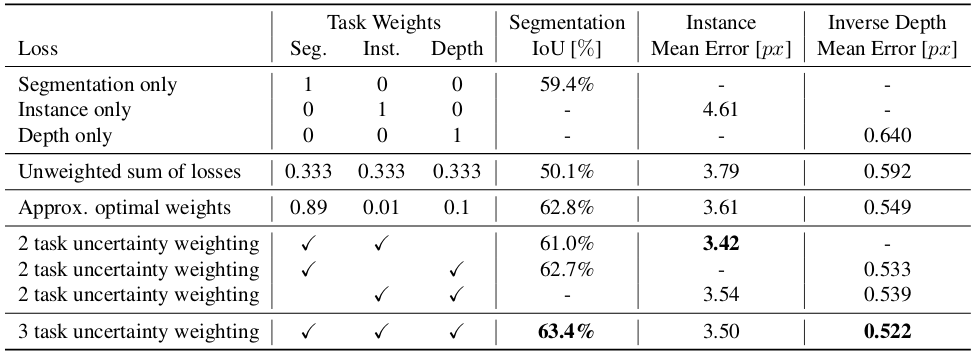
\includegraphics[width=1\linewidth]{data.png}
       % \end{tikzfigure}
        
    }
   
   
  
    \column{0.33} 
    \block{Reproduction results}{

   	
	\begin{itemize}
	\item Quantitative improvement for semantic segmentation and depth regression for multi-task model with learned weights
	\item Improved baseline for inverse mean depth error from 0.522 to 0.425
	\end{itemize}
	

	\begin{center}
   	\begin{tabular}{c c  c | c c c }
  	\hline			
  	  \multicolumn{3}{c|}{Task Weights} & $\:$ Segment. $\:$ &Instance Mean& $\:$ Inverse Depth$\:$ \\
	
	 $\:$Seg.$\:$ &$\:$ Inst.$\:$ &$\:$ Depth$\:$ & IoU [\%]&  $\:$ Error [$px$]$\:$  & $\:$ Mean Error [$px$]$\:$ \\
	\hline
  	 1 		& 0 	& 0			&33.2\% 	& -			&-\\
  	  0  	&  1 	& 0 		& -			&\textbf{5.27}	&-\\
	 0 		& 0 	&	1		&-			& -			& 0.446 \\ \hline 
	 0.333 & 0.333 & 0.333 		& 32.3\% 	& 5.72		& 0.459 \\
	 0.89 	&0.01	&0.1		&32.7 \%	&8.39		&0.528\\ \hline
	  $\!$ Learned $\!$ &	$\!$ Learned$\!$ 	& - 	&33.9\%		&7.17		& - \\
	 $\!$ Learned$\!$  & - &$\!$  Learned 	$\!$ 	& 33.2\% 	& - 		& 0.426 \\
	 - &$\!$  Learned $\!$ & $\!$ Learned $\!$ 		& - 		& 6.26		& 0.430 \\\hline
	 $\!$ Learned$\!$  &$\!$  Learned $\!$ & $\!$ Learned	$\!$ &\textbf{34.0\%} & 5.82 & \textbf{0.425} \\
 	 \hline  
	\end{tabular}
	
	

   \vspace{2em}
Ground truth \qquad \qquad \qquad \qquad \qquad  Predicted \quad
 
    \begin{tikzfigure}

    
    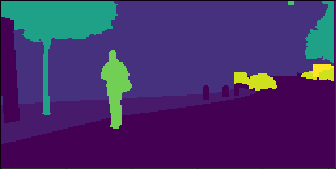
\includegraphics[width=0.49\linewidth]{semgt.png}
            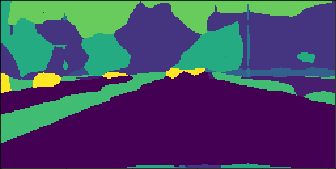
\includegraphics[width=0.49\linewidth]{sempred.png}
            
                Semantic segmentation
            \vspace{0.5em}
      
            
            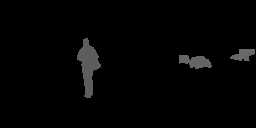
\includegraphics[width=0.49\linewidth]{instgt.png}
            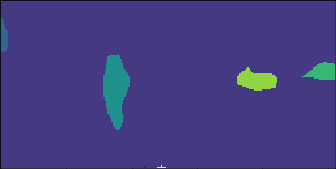
\includegraphics[width=0.49\linewidth]{instpred.png}
   
                  Instance segmentation
                  
               \vspace{0.5em}
              
               
             
\includegraphics[width=0.49\linewidth]{depgt.png}
              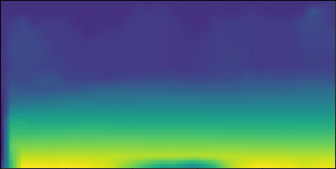
\includegraphics[width=0.49\linewidth]{deppred.png}
              
               Depth regression
        \end{tikzfigure}
	
	  	\end{center}
	
	
	%\begin{itemize}
	
	%\item Learning rate search

	%\begin{center}
   	%\begin{tabular}{c | c }
  	%\hline
	%$\>$Learning rate $\>$& $\>$Segmentation IoU $\>$\\			
  	%\hline
	%0.01 & \textbf{33.3}\%\\
	%0.001 & 33.0\%\\
	%0.0001 & 31.2\% \\
	%0.00001 & 25.2\% \\
 	 %\hline  
	%\end{tabular}
	%\end{center}
   %\vspace{0.5em}

    %\end{itemize} 
                    
    }

    
    \column{0.36}
    \block{Success on other multi-task problems}{
    
    \begin{itemize}
    \item Applying the principled approach to Fashion MNIST classification and reconstruction yields a learned weights multi-task model which outperforms individually trained models and fixed weights multi-task model
    
    \vspace{0.5em}
	\begin{center}
   	\begin{tabular}{c  c | c c }
  	\hline			
  	  \multicolumn{2}{c|}{Task weights} & $\>$ Classification $\>$ & $\>$ Reconstruction$\>$ \\
	
	 $\>$Classif.$\>$ &$\>$ Reconstr.$\>$ & accuracy [\%] & error \\
	\hline
  	 1  & 0  &89.7\% & -\\
  	  0  &  1& -& 0.087\\
	 0.5 & 0.5 &89.3\%& 0.085 \\ \hline 
	$\:$ Learned $\:$& $\:$ Learned $\:$& \textbf{90.2\%} & \textbf{0.075} \\
 	 \hline  
	\end{tabular}
	\end{center}
   \vspace{0.25em}
   
   \begin{tikzfigure}
            \includegraphics[width=0.7\linewidth]{clas}
             \includegraphics[width=0.7\linewidth]{reco}
        \end{tikzfigure}
	\item Reconstruction output sample from learned weights multi-task model
	  \vspace{-0.5em}
	
	\begin{tikzfigure}
            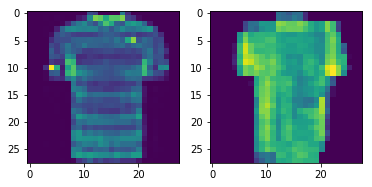
\includegraphics[width=0.7\linewidth]{shirt.png}
        \end{tikzfigure}
        
	%\item Optimal weight search
	
	%\begin{tikzfigure}
         %   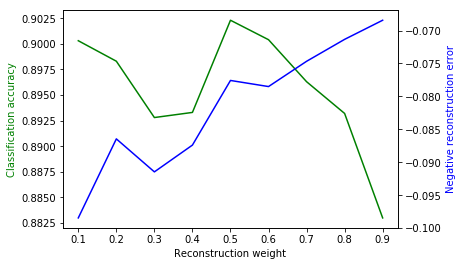
\includegraphics[width=0.8\linewidth]{optimal.png}
       % \end{tikzfigure}

   \end{itemize}   
    }
   
\end{columns}
\end{document}